\chapter{Gestió del projecte}
\label{ch:gestio}

En aquest capítol es descriu el marc metodològic utilitzat per al desenvolupament del projecte, la planificació temporal detallada de les tasques i l'anàlisi econòmica i de sostenibilitat del sistema.

\section{Metodologia i eines de treball}
El projecte es desenvolupa en un entorn professional dins de l’equip d’\textit{Embedded} de Lanaccess. S’ha optat per una \textbf{metodologia àgil basada en Kanban}, utilitzant l'eina \textit{Businessmap} per a la gestió visual del flux de treball. Aquesta elecció permet una gran flexibilitat i una resposta ràpida davant de canvis en els requeriments tècnics.

Els pilars del seguiment del projecte són:
\begin{itemize}
    \item \textbf{Reunions de sincronització (Daily):} Sessions diàries per coordinar el progrés, identificar bloquejos i alinear el \textit{frontend} amb l'estat del \textit{firmware}.
    \item \textbf{Seguiment acadèmic i professional:} El director del TFG supervisa l'evolució tècnica diàriament, mentre que es manté una comunicació constant amb el tutor de la universitat per garantir el rigor acadèmic.
    \item \textbf{Gestió de tasques:} Control del cicle de vida de cada funcionalitat des de la columna \textit{To Do} fins a \textit{Done}.
\end{itemize}

Respecte a l'enginyeria de software, se segueixen els estàndards següents:
\begin{itemize}
    \item \textbf{Control de versions:} Ús de \textbf{Git} amb el model \textbf{GitFlow} (branques \textit{master}, \textit{develop} i \textit{feature}). El repositori es troba allotjat en un GitLab local.
    \item \textbf{Stack tecnològic:} Angular 19 (Signals i Standalone Components) per al \textit{frontend} i implementacions en C++ 22 per a la comunicació de baix nivell en el \textit{backend}.
    \item \textbf{Qualitat:} Aplicació de principis SOLID i arquitectura modular.
\end{itemize}

\section{Planificació temporal}

\subsection{Descripció de les fases i tasques}
El projecte s'estructura en sis fases lògiques pactades amb l'empresa:

\begin{enumerate}
    \item \textbf{Gestió i Formació (GF):} Inclou l'autoformació en Angular 19 i la gestió administrativa de l'assignatura GEP.
    \item \textbf{Mòdul d'Autenticació i Core (AC):} Desenvolupament del \textit{login}, la \textit{home page} i el sistema base de \textit{logs} i alertes.
    \item \textbf{Manteniment i Configuració Base (MC):} Gestió de llicències, actualització de \textit{firmware} i integració del motor de base de dades.
    \item \textbf{Alarmes i Sistema de Vídeo Directe (AV):} Implementació del motor d'alarmes via WSS i visualització en temps real.
    \item \textbf{Mòdul de Gravacions i Configuració Avançada (GV):} Reproducció d'històrics (HLS) i motor de configuració dinàmica \textit{Schema-driven}.
    \item \textbf{Finalització i Memòria (FM):} Fase de correcció d'errors, repàs de qualitat i redacció final.
\end{enumerate}

\subsection{Recursos identificats}
Per a l'execució del projecte es requereixen els següents recursos:
\begin{itemize}
    \item \textbf{Humans (Rols):} Cap de Projecte (planificació), Analista (disseny d'arquitectura), Programador (codificació) i Tester (validació).
    \item \textbf{Materials:} Ordinador portàtil (ASUS Expertbook), videogravador Lanaccess de proves i espai de despatx equipat.
    \item \textbf{Software:} VS Code, Git, Angular 19, RxJS i llibreries de vídeo (WebRTC, HLS.js).
\end{itemize}

\subsection{Estimació d'hores i Diagrama de Gantt}
S'ha estimat una càrrega total de \textbf{540 hores} (18 ECTS). La Taula \ref{tab:estimacio_hores} resumeix el repartiment temporal segons el planning oficial.

\begin{table}[htbp]
\centering
\caption{Estimació d'hores i dependències de les tasques.}
\label{tab:estimacio_hores}
\small
\begin{tabular}{@{}llllc@{}}
\toprule
\textbf{ID} & \textbf{Tasca} & \textbf{Mes/Setmana} & \textbf{Dependència} & \textbf{Hores} \\ \midrule
GF1 & Formació Angular 19 & Desembre & - & 40 \\
AC1 & Login & Gener S1 & GF1 & 20 \\
AC2 & Home Page & Gener S2 & AC1 & 20 \\
AV1 & Core Alarm (WSS) & Feb S4 - Mar S1 & AC3 & 50 \\
AV3 & Càmeres Directe & Març S3 - S4 & AC2 & 50 \\
GV2 & System Config Avançat & Abr S3 - Maig S1 & MC2 & 60 \\
FM2 & Memòria TFG & Transversal & - & 80 \\ \midrule
\textbf{TOTAL} & & & & \textbf{540} \\ \bottomrule
\end{tabular}
\par\smallskip
\small Font: Elaboració pròpia.
\end{table}

\newpage
% --- AQUÍ POSES LA TEVA IMATGE DEL GANTT ---
\begin{figure}[htbp]
    \centering
    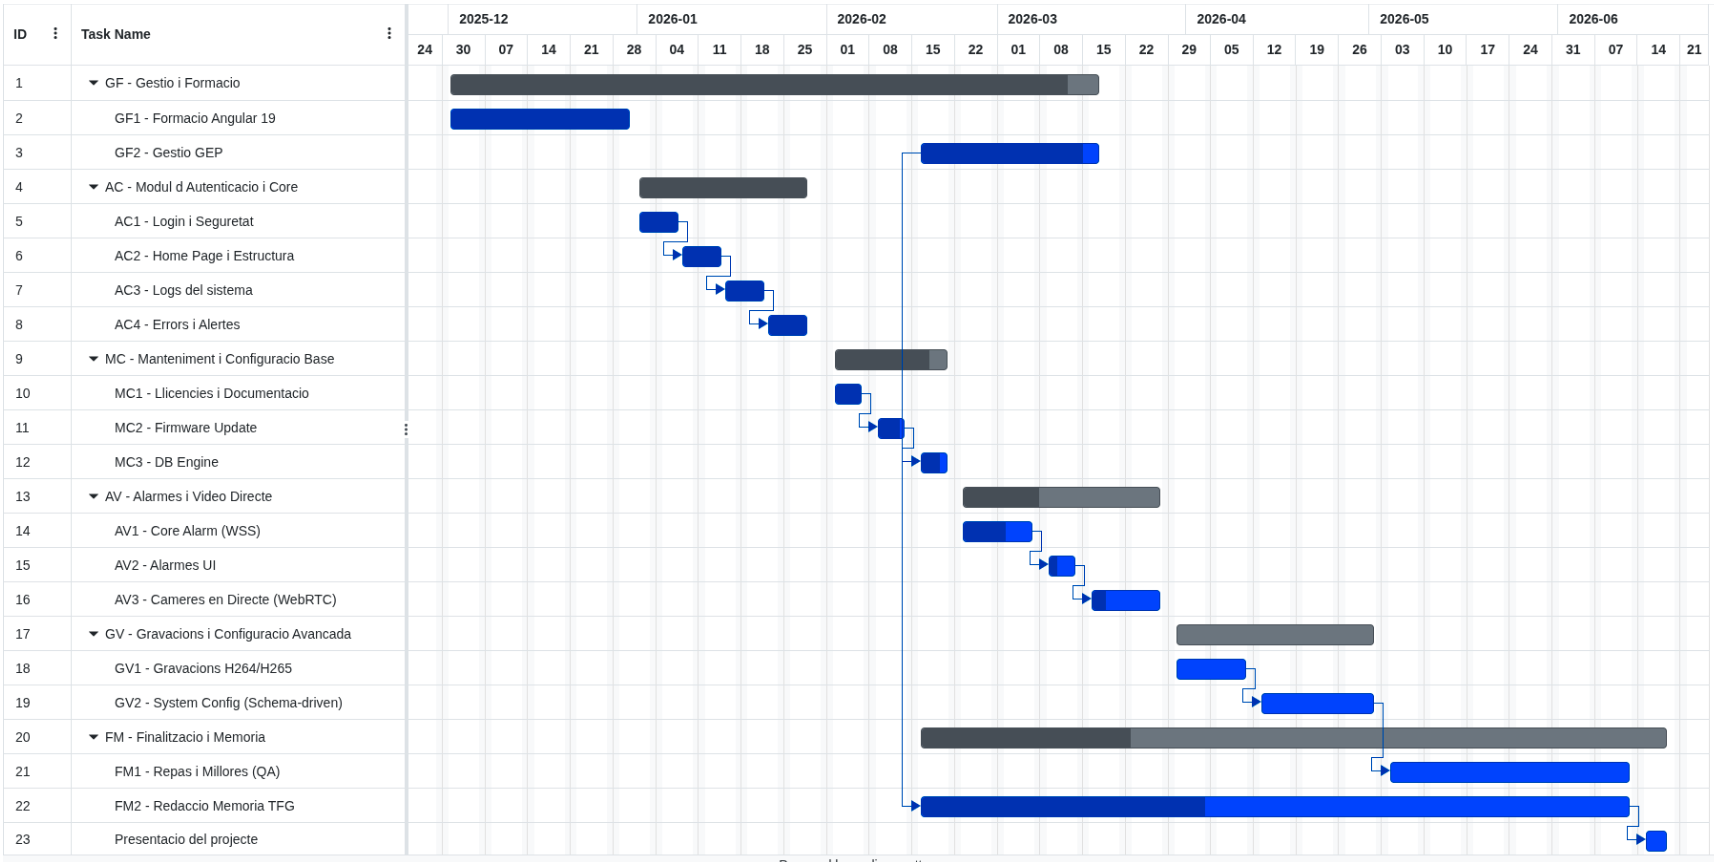
\includegraphics[width=1\textwidth]{figures/gantt.png}
    \caption{Diagrama de Gantt del projecte.}
    \label{fig:gantt}
    \small Font: Elaboració pròpia.
\end{figure}

\subsection{Gestió del risc i desviacions reals}
S'han previst plans de contingència per a retards en la formació o incompatibilitats en els protocols de vídeo (WebRTC). Actualment, s'han detectat desviacions en [completar amb la teva experiència real, ex: la implementació del motor WebRTC per problemes de latència].

\section{Anàlisi econòmica}
L'estimació econòmica s'ha realitzat assumint rols professionals i preus de mercat actuals, afegint un factor d'1,35 per cobrir la Seguretat Social.

\subsection{Costos de personal}
\begin{table}[htbp]
\centering
\caption{Costos de recursos humans per rol.}
\label{tab:costos_humans}
\begin{tabular}{@{}lcccc@{}}
\toprule
\textbf{Rol} & \textbf{Sou Brut/h (€)} & \textbf{Cost Real/h (€)} & \textbf{Hores} & \textbf{Total (€)} \\ \midrule
Project Manager & 25,00 & 33,75 & 90 & 3.037,50 \\
Analista & 20,00 & 27,00 & 100 & 2.700,00 \\
Programador & 18,00 & 24,30 & 250 & 6.075,00 \\
Tester & 13,00 & 17,55 & 100 & 1.755,00 \\ \midrule
\textbf{TOTAL CPA} & & & \textbf{540} & \textbf{13.567,50} \\ \bottomrule
\end{tabular}
\end{table}

\subsection{Costos totals i control de gestió}
Sumant l'amortització del hardware (210,00 €), els costos indirectes \- d'oficina (1.150,00 €) i un marge de contingència del 10 \%, el pressupost final estimat és de \textbf{16.810,40 €}.

El control de gestió es realitza mitjançant la fórmula de desviació de costos:
\[ \text{Desviació} = (\text{Hores Planificades} - \text{Hores Reals}) \times \text{Cost/h} \]

\section{Informe de sostenibilitat}
\begin{itemize}
    \item \textbf{Dimensió Econòmica:} La solució \textit{Schema-driven} permet adaptar el software a nous models de gravadors sense cost addicional, allargant la vida útil del producte.
    \item \textbf{Dimensió Ambiental:} L'ús de la plataforma web redueix els desplaçaments físics de tècnics a les instal·lacions del client, minimitzant la petjada de carboni.
    \item \textbf{Dimensió Social:} Millora la interfície de treball dels operadors de seguretat, reduint l'estrès operatiu en situacions d'incident crític.
\end{itemize}